 
\documentclass[a4paper,12pt]{article}
\usepackage[pstricks]{sk2}


\author{Groupe CRT 1\\Développement}

\title{Rapport de projet}

\def\tech{\texttt}

% name formatting
\def\familyname{\textsc}
\def\firstname#1{#1}
\def\groupmember#1#2{\firstname{#1} \familyname{#2}}

% group members
\def\mwyd{\groupmember{Wydade}{Ben Hamdia}}
\def\mmat{\groupmember{Mathias}{Coqblin}}
\def\mlou{\groupmember{Loubna}{Darkate}}
\def\mmor{\groupmember{Mor Salla}{Fall}}
\def\moli{\groupmember{Olivier}{Finot}}
\def\mvin{\groupmember{Vincent}{Hugot}}
\def\mmed{\groupmember{Mehdi}{Iraqi Houssaini}}
\def\mbed{\groupmember{Bedr}{MOUAJAB}}
\def\mdon{\groupmember{Donald}{Srey}}

\def\grpd{Groupe Développement}
\def\grpt{Groupe Test}

\begin{document}
 
\maketitle


\tableofcontents


\section{Réunion initiale (zéro): 2009-09-30}

Durant cette première réunion durant le TP de CRT, nous 
nous sommes répartis en deux sous-groupes, l'un dédié au développement
de l'application, et l'autre au test.\mk\\
%
La répartition nominative de ces groupes est la suivante:
\begin{itemize}
\item \mvin : Chef de projet, chef \grpd
\item \mmat
\item \moli
\item \mbed
\item \mmed
\end{itemize}


\begin{itemize}
\item \mwyd : Chef \grpt
\item \mdon
\item \mlou
\item \mmor
\end{itemize}


\noi Les tâches définies pour l'itération étaient:

\begin{itemize}
 \item \moli\ et \mmat: Création (sur papier pour l'instant) d'un modèle objet cohérent sur lequel fonder le développement.
\item  \mvin : Définition du langage d'entrée et écriture d'un parseur complet pour ce langage.
\item Le \grpt, et d'une manière générale tout personne n'ayant pas de tâche précise,
était chargé de se documenter sur les outils de test
unitaire, plugins \texttt{Eclipse} dédiés aux tests etc
\end{itemize}
La raison pour laquelle tout le monde n'avait pas de tâche précise est que la 
quasi-totalité des tâches de développement dépendent du modèle, lequel n'était 
pas encore défini.\mk\\
%
Ce document étant le rapport du \grpd, les tâches du \grpt\ seront
omises dans les sections suivantes.

\section{Première réunion: 2009-10-6}

\subsection{Bilan de l'itération passée}

\begin{itemize}
 \item \moli\ et \mmat\ ont présenté leur proposition de modèle, qui a été acceptée. 
  Ci-dessous, le brouillon
 de diagramme UML utilisé lors de cette réunion. Il est à noter que les choses ont 
 évolué depuis, et qu'il ne reflète pas nécessairement la structure actuelle du système. 

  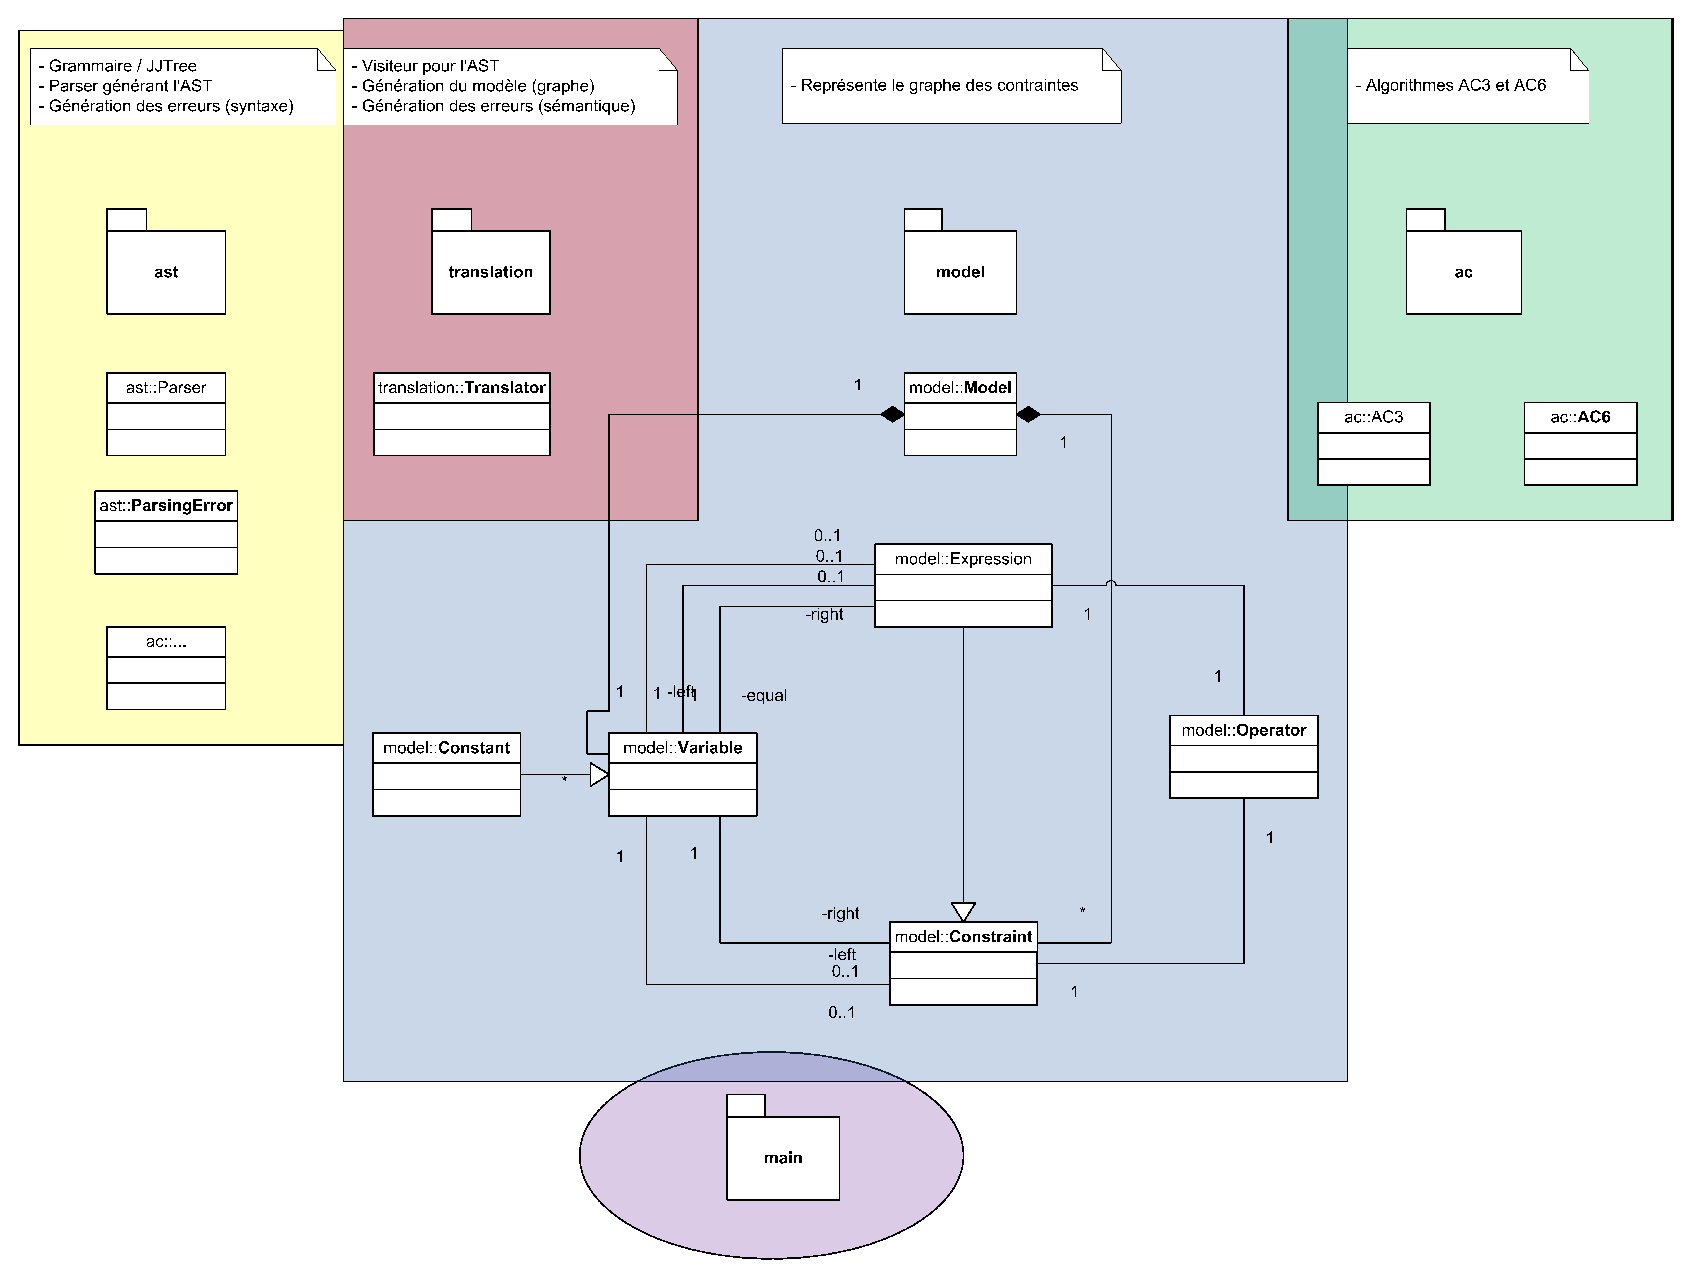
\includegraphics[scale=0.4]{uml.eps}
\item \mvin\ a présenté le parseur; Le fichier \texttt{jjt} proposé,
  insuffisant pour de nombreuses raisons, n'a pas été conservé. 
  Ce commentaire extrait du fichier \texttt{parser.jjt} donne
  une liste non-exhaustive des avantages du parseur réalisé
  en comparaison de celui qui nous était proposé:
\begin{verbatim}
/** 
 * Parser for the constraints.
 * by Vincent Hugot, 2009-10-4
 
 * This grammar has the following advantages over the one 
     which was suggested:
 
  * More robust: Won't die if there are too many line feeds 
     at the beginning or end...
  * Support for negative integers (the other did not!!)
  * AST expression trees correspond to the intuitive idea:
    +(2,3) instead of Exp(2,Exp(+,3)); visitors will be much
    easier to implement...
  * Expressions are (correctly) left-associative
  * Expressions support operator priorities
  * Supports parentheses to override priorities
    (the other had no priorities and no parens to 
    explicitely specify them... the only possible way 
    to get correct nesting would
    have been to introduce intermediary variables... a mess !)
  * Supports several constraints on one line, comma-separated
     
 * ... and the following difference
  * Domains must be grouped at beginning of file
    (can be seen as a restriction; 
     I see it as a cleaner way of doing things but YMMW)
  
**/
\end{verbatim}
\end{itemize}



\subsection{Tâches pour la prochaine itération}

\begin{itemize}
 \item \mmed\ a été chargé de se documenter sur les algorithmes AC3 et AC6,
afin de pouvoir donner une présentation à la prochaine réunion et
préparer le terrain pour l'implantation des algorithmes vis-à-vis du 
modèle.
\item \mvin\ et \mbed\ ont été chargés d'implanter une phase de 
 vérification/typechecking pour filtrer les erreurs
 les erreurs qui peuvent être détectées statiquement afin
 de garantir la production d'un modèle cohérent.
\item \moli\ et \mmat\ ont été chargés d'implanter le modèle
\end{itemize}








\section{Seconde réunion: 2009-10-14}

\subsection{Bilan de l'itération passée}

\begin{itemize}
 \item \mvin\ et \mbed\ ont implanté un visiteur de typechecking, 
  qui détecte statiquement les erreurs qui peuvent l'être, 
  par exemple les redéfinitions sauvages de variables, les utilisations
  de variables non définies etc. 
\item \moli et \mmat\ ont totalement implanté le modèle.
\item \mmed\ a présenté des éléments sur l'algorithme AC3.
\end{itemize}


\subsection{Tâches pour la prochaine itération}

\begin{itemize}
 \item \mmat\ et \mvin\ ont été chargés d'implanter un visiteur
de traduction, dont le but est de générer un modèle à partir 
d'un arbre de syntaxe abstraite issu du parseur.

\item \mbed\ et \mmed\ ont été chargés d'implanter AC3. \moli\
était chargé, parallèlement, de rajouter au modèle
toutes méthodes dont ils pourraient avoir besoin lors de
l'implantation de l'algorithme et qui n'auraient pas
déjà été implantées.

\end{itemize}



\section{Troisième réunion: 2009-10-21}

\subsection{Bilan de l'itération passée}

\begin{itemize}
 \item \mmed\ et \mbed\ ont implanté (mais non testé) une pré-version de 
 l'algorithme AC3, qui a été critiquée en détail par \mvin\ et \mmat, et très
 largement remanié par ce dernier.
 A noter que l'algorithme, à ce stade, ne prenait pas encore en compte la
 propagation des restrictions de domaine aux substitutions.
\item \moli\ a rajouté quelques méthodes au modèle pour le rendre plus aisément
manipulable par les algorithmes.
\item \mmat\ a implanté le visiteur de traduction.
\end{itemize}


\subsection{Tâches pour la prochaine itération}

Il a été décidé de travailler pendant les vacances. Un programme
et une répartition des tâches ont été suggérés, mais nous ne nous y sommes pas 
tenus\dots

\section{Quatrième réunion: 2009-10-30}

Réunion pendant les vacances, faisant le bilan du travail
effectué pendant les premiers jours de "vacances".

\subsection{Bilan de l'itération passée}

\begin{itemize}
 \item \mmat\ a remanié AC3 de manière à répercuter les restrictions de domaines aux
 substitutions. 
\item \moli\ a implanté AC6 (sans support des substitutions)
\item \mvin\ a implanté une méthode \texttt{main} permettant de piloter le programme
  en ligne de commande; ajouté une classe \tech{Domain} permettant
  de centraliser les calculs effectués sur les domaines des substitutions,
  c'est à dire les opérations arithmétiques sur les domaines. 
  Ces opérations étaient auparavant dupliquées un peu partout dans le
  code des algorithmes et du visiteur de traduction.
  Il a également ajouté une méthode permettant d'exporter 
  un diagramme \LaTeX\ \texttt{\emph{PStricks}} représentant un domaine
  de manière graphique. Ceci est un compromis entre réaliser
  une interface graphique, ce qui n'était pas demandé et
  prendrait trop de temps, et rester uniquement en mode texte,
  ce qui ne facilite pas toujours la visualisation des résultats.
  Ci-après, un modèle et sa représentation graphique générée:
  \begin{verbatim}
DOMAINS:
  A : [1, 2, 3, 4, 5]
  C : [8, 9]
  B : [1, 2, 3]
  @1 : [8, 9, 16, 18, 24, 27]
  @2 : [9, 10, 11, 12, 13, 14]
  42 : [42]
  56 : [56]
CONSTRAINTS:
  A < @1
  B <= @2
  A > C
  B >= C
  42 != 56
  A = B
SUBSTITUTIONS:
  @1 = B * C
  @2 = C + A
  \end{verbatim}


\pspicture(-5.0766680269147635,-5.0766680269147635)(5.0766680269147635,5.0766680269147635)
%%CRT to LaTeX: ; 2.0; 3.5; 0.51; 0.01
%%VAR: A : [1, 2, 3, 4, 5]
\rput(2.294709574895252,1.1305587958113439){\rnode{A}{\psshadowbox{\bf A}}}
\rput(4.476487689584901,0.04018193867599526){\rnode{@@DOMA}{\psframebox[framearc=.4]{\scriptsize $\{1..5\}$}}}
\ncline[linestyle=solid]{*-*}{A}{@@DOMA}
%%VAR: C : [8, 9]
\rput(0.5468215588283258,2.4989680683640008){\rnode{C}{\psshadowbox{\bf C}}}
\rput(2.7596289179188567,3.5249120355814445){\rnode{@@DOMC}{\psframebox[framearc=.4]{\scriptsize $\{8,9\}$}}}
\ncline[linestyle=solid]{*-*}{C}{@@DOMC}
%%VAR: B : [1, 2, 3]
\rput(-1.612834244163338,1.985603415779802){\rnode{B}{\psshadowbox{\bf B}}}
\rput(-1.0352867151111822,4.355311474592285){\rnode{@@DOMB}{\psframebox[framearc=.4]{\scriptsize $\{1..3\}$}}}
\ncline[linestyle=solid]{*-*}{B}{@@DOMB}
%%VAR: @1 : [8, 9, 16, 18, 24, 27]
\rput(-2.5579929654770863,-0.022961107814853665){\rnode{@1}{\psshadowbox{\bf @1$\times$}}}
\rput(-4.050610335662157,1.9060725410717807){\rnode{@@DOM@1}{\psframebox[framearc=.4]{\scriptsize $\{8,9,16,18,24,27\}$}}}
\ncline[linestyle=solid]{*-*}{@1}{@@DOM@1}
%%VAR: @2 : [9, 10, 11, 12, 13, 14]
\rput(-1.5769308102393478,-2.0142354489036824){\rnode{@2}{\psshadowbox{\bf @2$+$}}}
\rput(-4.015741756066691,-1.9784778926698503){\rnode{@@DOM@2}{\psframebox[framearc=.4]{\scriptsize $\{9..14\}$}}}
\ncline[linestyle=solid]{*-*}{@2}{@@DOM@2}
%%VAR: 42 : [42]
\rput(0.5915924086349604,-2.4887494140527346){\rnode{42}{\psshadowbox{\bf 42}}}
\rput(-0.9569377279495715,-4.373194119637){\rnode{@@DOM42}{\psframebox[framearc=.4]{\scriptsize $\{42\}$}}}
\ncline[linestyle=solid]{*-*}{42}{@@DOM42}
%%VAR: 56 : [56]
\rput(2.3146344775212326,-1.089184309183875){\rnode{56}{\psshadowbox{\bf 56}}}
\rput(2.8224599272858413,-3.4748059776146536){\rnode{@@DOM56}{\psframebox[framearc=.4]{\scriptsize $\{56\}$}}}
\ncline[linestyle=solid]{*-*}{56}{@@DOM56}
\psset{arrowscale=2}
%%CON: A < @1
\ncarc[doubleline=false,linestyle=solid]{<-}{A}{@1}
%%CON: B <= @2
\ncarc[doubleline=true,linestyle=solid,arrowscale=1]{<-}{B}{@2}
%%CON: A > C
\ncarc[doubleline=false,linestyle=solid]{->}{A}{C}
%%CON: B >= C
\ncarc[doubleline=true,linestyle=solid,arrowscale=1]{->}{B}{C}
%%CON: 42 != 56
\ncarc[doubleline=true,linestyle=dashed,arrowscale=0.8]{|-|}{42}{56}
%%CON: A = B
\ncarc[doubleline=true,linestyle=dashed]{-}{A}{B}
%%SUB: @1 = B * C
\ncline[linestyle=dotted,arrowscale=1.35]{*-}{@1}{B}
\ncline[linestyle=dotted,arrowscale=1.35]{o-}{@1}{C}
%%SUB: @2 = C + A
\ncline[linestyle=dotted,arrowscale=1.35]{*-}{@2}{C}
\ncline[linestyle=dotted,arrowscale=1.35]{o-}{@2}{A}
\endpspicture
\end{itemize}


\subsection{Tâches pour la prochaine itération}

\`A ce stade, le développement était presque terminé, puisqu'il
 ne restait plus qu'à ajouter le support des substitutions à AC6.\mk\\
%
Les réunions qui ont suivi ont été principalement consacrées à
la discussion avec l'équipe de test sur Fitnesse.


\section{Dernière réunion/séance de développement: 2009-11-27}

Nous avons appris au dernier moment que nous devions réaliser 
un algorithme de backtracking; le besoin de rédiger un rapport
(bien que peu surprenant) était également une addition récente.
La répartition des tâches sur cette dernière séance de 
travail était donc comme suit: 
\begin{itemize}
 \item \mmat\ s'est chargé de l'algorithme de backtracking
\item \mvin\ s'est chargé d'exhumer les rapports de réunion pour
rédiger le présent rapport.
\item \moli\ s'est chargé de continuer le travail sur AC6.
\end{itemize}

\section{Remarque générale}

Le travail de développement s'est fait relativement rapidement, 
le plupart du temps par petits groupes de travail (binômes ou trinômes).
Les séances de développement se faisant souvent dans la même salle,
en particulier pendant les vacances,
il y avait beaucoup de communication entre les différents groupes de travail,
de sorte que les développeurs ont souvent 
participé à d'autres aspects que ceux qui leur avaient été spécifiquement
confiés.



\end{document}
